\section{GLOSARIO}
\begin{frame}{GLOSARIO}
	\begin{itemize}
		\item Tee (de salida): Lugar del hoyo de golf donde los golfistas comienzan el juego en cada hoyo.
  	    \item Down swing: Bajada del palo que comienza desde lo alto del back swing hasta el momento del impacto de la cara del palo en la bola de golf.
        \item Backswing: Es la parte del swing de golf en la que elevamos el palo. Comienza cuando arrancamos la cabeza del palo en el inicio del swing y termina en lo alto de la subida del palo.
        \item Swing: Movimiento que empleamos para golpear la bola de golf 
        
            \item Grip (mango): Mango de goma situado en la varilla de los palos de golf, con la finalidad de facilitar su agarre. Existen diferentes tipos y grosores, en función de los jugadores o jugadoras a los que van destinados\footnote{\bibentry{bworld}}.
        \item Número de Reynolds: Se utiliza para estudiar la manera en que se comporta el fluido al rededor de un objeto en movimiento; en particular, para determinar si el flujo es laminar o turbulento\footnote{\bibentry{reynolds}}.
	\end{itemize}
\end{frame}
%%%%%%%%%%%%%%%%%%%%%%%%%%%%%%
\begin{frame}{GLOSARIO}
\begin{itemize}
			\item Hook: Efecto pronunciado hacia la izquierda que toma la bola de golf durante el vuelo, a consecuencia de llegar la cara del palo cerrada en el momento del impacto.
            \item Slice: Efecto pronunciado hacia la derecha que toma la bola de golf durante el vuelo, a consecuencia de llegar la cara del palo abierta en el momento del impacto.
            \item Backspin: Efecto de retroceso que se imprime al golpear la bola. Cuando impacta en el green, regresa en sentido opuesto a la trayectoria del golpe.
            \item Overspin: opuesto al backspin\footnote{\vspace{-0.3cm}\bibentry{bworld}}.
\end{itemize}
    \begin{figure}[H]
      \centering
      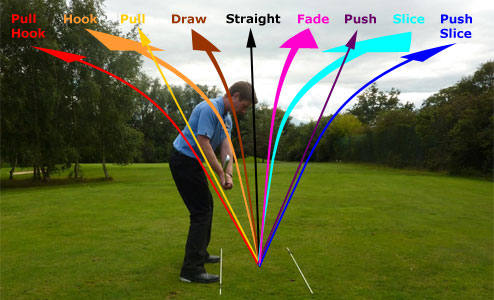
\includegraphics[scale = 0.35]{Spin_Shots.jpg}
      \caption{Tipos de tiro en el golf.}
	\end{figure}
\end{frame}








